%%%%%%%%%%%%%%%%%%%%%%%%%%%%%%%%%%%%%%%%%%%%%%%%%%%%%%%%%%%%%%%%%%%%%%
%%%%%%%%%%%%%%%%%%%%%%%%%%%%%%%%%%%%%%%%%%%%%%%%%%%%%%%%%%%%%%%%%%%%%%
% BAB HASIL DAN PEMBAHASAN:
%=====================================================================
\renewcommand{\thechapter}{\Roman{chapter}}
\addtocontents{toc}{\vskip10pt}
\chapter{HASIL DAN PEMBAHASAN}
\renewcommand{\thechapter}{\arabic{chapter}}
%---------------------------------------------------------------------

%=====================================================================
\section{Pra-Kalkulasi Sifat Elektronik}
%=====================================================================
Sebelum dilakukannya proses kalkulasi untuk struktur pita dan rapat keadaan, kita harus memastikan bahwa parameter-parameter yang kita gunakan sudah sesuai dan efisien dari segi waktu dan biaya komputasi. Salah satu parameter penting dalam input perhitungan DFT kami ialah \textit{cutoff} energi kinetik dan K-POINTS. Kedua parameter ini perlu diselidiki kekonvergenannya. Selain itu struktur yang digunakan harus dalam konfigurasi dengan tingkat energi paling rendah (stabil). Dalam pra-kalkulasi di bawah akan ditentukan parameter \texttt{ecutwfc}, \texttt{K-POINTS}, dan optimasi struktur \texttt{vc-relax}.\nocite{Giannozzi_2017}\nocite{giannozzi2020quantum}

%=====================================================================
\subsection{Konvergensi \textit{cutoff} Energi Kinetik (\texttt{ecutwfc})}
%=====================================================================
Salah satu input terpenting dalam Quantum ESPRESSO \textit{cutoff} adalah energi kinetik. Dalam Quantum ESPRESSO, fungsi gelombang elektron diaproksimasi dalam basis gelombang datar \textit{(plane wave basis)}\citep{DFTSholl}. \textit{Cutoff} Energi kinetik menentukan jumlah maksimum gelombang datar yang digunakan dalam perhitungan. Semakin tinggi \textit{cutoff} energi kinetik, semakin banyak gelombang datar yang digunakan, yang dapat meningkatkan presisi perhitungan. Namun, peningkatan ini juga akan meningkatkan kompleksitas dan waktu komputasi. Pemilihan \textit{cutoff} energi kinetik harus mempertimbangkan keseimbangan antara kepresisian hasil yang diinginkan dan biaya komputasi yang dapat diterima. Jika \textit{cutoff} energi kinetik terlalu rendah, hasil perhitungan dapat menjadi tidak akurat. Di sisi lain, jika \textit{cutoff} energi kinetik terlalu tinggi, waktu komputasi dapat menjadi lebih lama dan tidak efisien. Dalam sistem periodik, fungsi gelombang bidang dieksoresikan sebagai \citep{Giannozzi_2009}
\begin{equation}
    \psi (\textbf{r}) = \frac{1}{\Omega} \sum_\textbf{G} c_{\textbf{k},\textbf{G}} e^{i(\textbf{k}+\textbf{G})\cdot\textbf{r}}
\end{equation}
di mana \textbf{G} adalah vektor kisi resiprok. Gelombang bidang ini dapat direpresentasikan sebagai sebuah \textit{grid} (kisi) dalam bidang-k (\textit{k-plane}). Semakin banyak grid yang kita gunakan, akan semakin akurat hasil kalkulasi yang kita jalankan, namun akan menambah biaya dan efisiensi kalkulasi. Secara prinisp, jumlah gelombang bidang yang memenuhi perioditas material adalah tak hingga dan tidak mungkin bagi kita menghitung gelombang bidang sebanyak itu. Oleh karena itu kita harus membatasi jumlah gelombang bidang yang akan kita hitung dengan cara membatasi panjang gelombang minimum $\lambda_{min}$ dalam ruang vektor. Penentuan panjang panjang gelombang minimun berkorespondensi terhadap bentuk maksimum vektor gelombang pada ruang vektor sebagai berikut,
\begin{equation}
    |\textbf{G}_{max}|= \frac{2\pi}{\lambda_{min}}
\end{equation}
Kemudian dari persamaan (4.2) dapat dibentuk definisi dari \textit{cutoff} energi kinetik sebagai berikut
\begin{equation}
    E_{cut}=\frac{\hbar^2}{2m} |\textbf{G}_{max}|
\end{equation}
dan kita membatasi \textit{cutoff} energi dengan batasan sebagai berikut
\begin{equation}
    \frac{\hbar|\textbf{k}+\textbf{G}|}{2m}\le E_{cut}
\end{equation}
jadi dengan menentukan \textit{cutoff} energi kinetik secara tidak lansung kita menentukan panjang gelombang minimum pada ruang vektor yang berkorespondensi dengan jumlah gelombang bidang yang akan kita gunakan dalam kalkulasi.

Dalam penelitian ini, dilakukan perhitungan SCF dengan beberapa variasi \texttt{ecutwfc}. seperti yang terlihat pada gambar 4.1 energi total mulai konvergen ketika \texttt{ecutwfc} bernilai 30 Rydberg jadi untuk kepresisian dan efisiensi kalkulasi, penulis menggunakan \texttt{ecutwfc} sebesar 60 Rydberg. nilai \texttt{ecutwfc} diambil karena merupakan saran dari sumber \textit{pseudopotential} SSSP Materials Cloud. Sedangkan untuk input \texttt{ecutrho} penulis menggunakan nilai \textit{default} 480 Rydberg \texttt{ecutwfc} dengan saran dari sumber \textit{pseudopotential} yang sama.

\begin{figure}
    \centering
    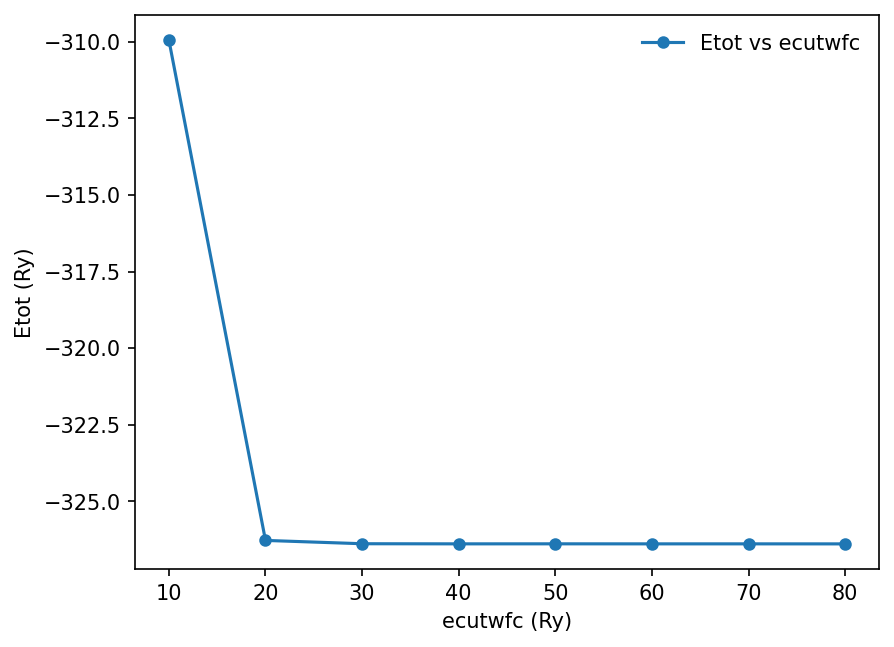
\includegraphics[width=15cm]{./gambar/plot_ecut_sn.png}
    \caption{Konvergensi \textit{cutoff} energi kinetik}
    \label{fig:ecutwfc}
\end{figure}



%-------------------------------------------------------------------


%=====================================================================
\subsection{Konvergensi \texttt{K-POINT}}
%=====================================================================
\texttt{K-POINT} mengacu pada titik-titik dalam ruang momentum yang digunakan dalam perhitungan untuk merepresentasikan distribusi elektron dalam struktur kristal. Sama halnya dengan \texttt{ecutwfc} Pemilihan \texttt{K-POINTS} mempengaruhi akurasi dan kecepatan perhitungan.
\begin{figure}
    \centering
    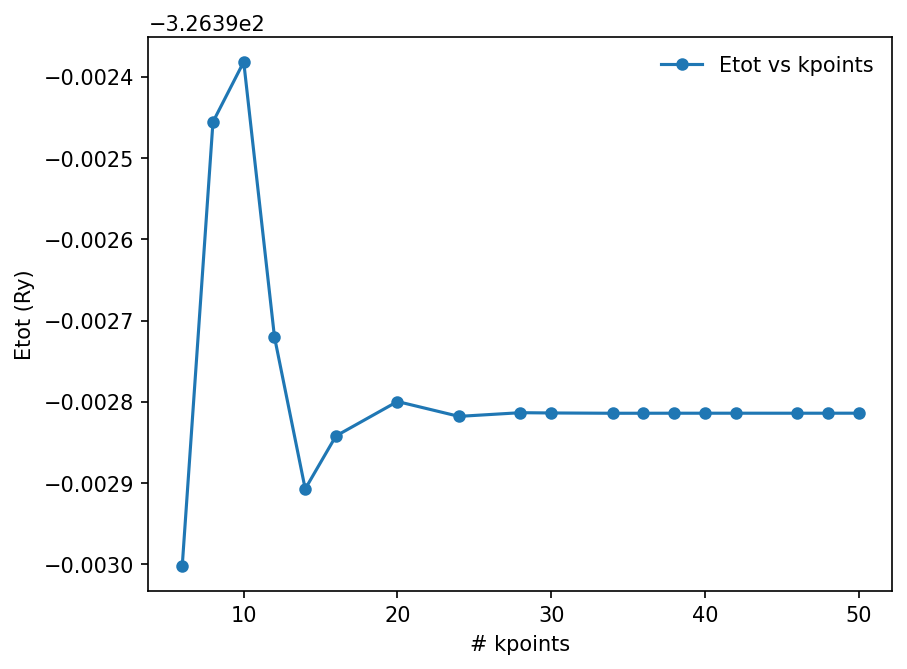
\includegraphics[width=15cm]{./gambar/plot_kpoints_sn.png}
    \caption{Konvergensi K-points}
    \label{fig:kpoints}
\end{figure}
Dalam metode DFT yang digunakan oleh Quantum ESPRESSO, distribusi elektron dalam struktur kristal diwakili oleh fungsi gelombang Bloch. Fungsi gelombang ini diekspansi dalam basis gelombang datar (\textit{plane wave basis}) dan faktor fase Bloch. Titik-titik k dalam ruang momentum menentukan faktor fase Bloch dan mewakili kontribusi dari setiap bagian dalam \textit{Brillouin Zone} (BZ). Dalam penelitian kali ini, nilai energi total mulai konvergen pada variasi \texttt{K\_POINT} $18\times18\times1$. Namun, untuk meningkatkan akurasi, penulis menggunakan variasi $24\times24\times1$ untuk struktur \textit{stanene}

\subsection{Optimasi Struktur (\texttt{vc-relax})}
Optimasi struktur input kita dilakukan melalui perhitungan Perhitungan \texttt{vc-relax} dalam Quantum ESPRESSO adalah perhitungan yang digunakan untuk mengoptimalkan struktur kristal dalam keadaan yang rileks secara volumetrik dan sel yang rileks. "vc" dalam \texttt{vc-relax} adalah singkatan dari \textit{volume and cell}, yang menunjukkan bahwa perhitungan ini memperhatikan optimisasi volume dan sel.
\begin{figure}
    \centering
    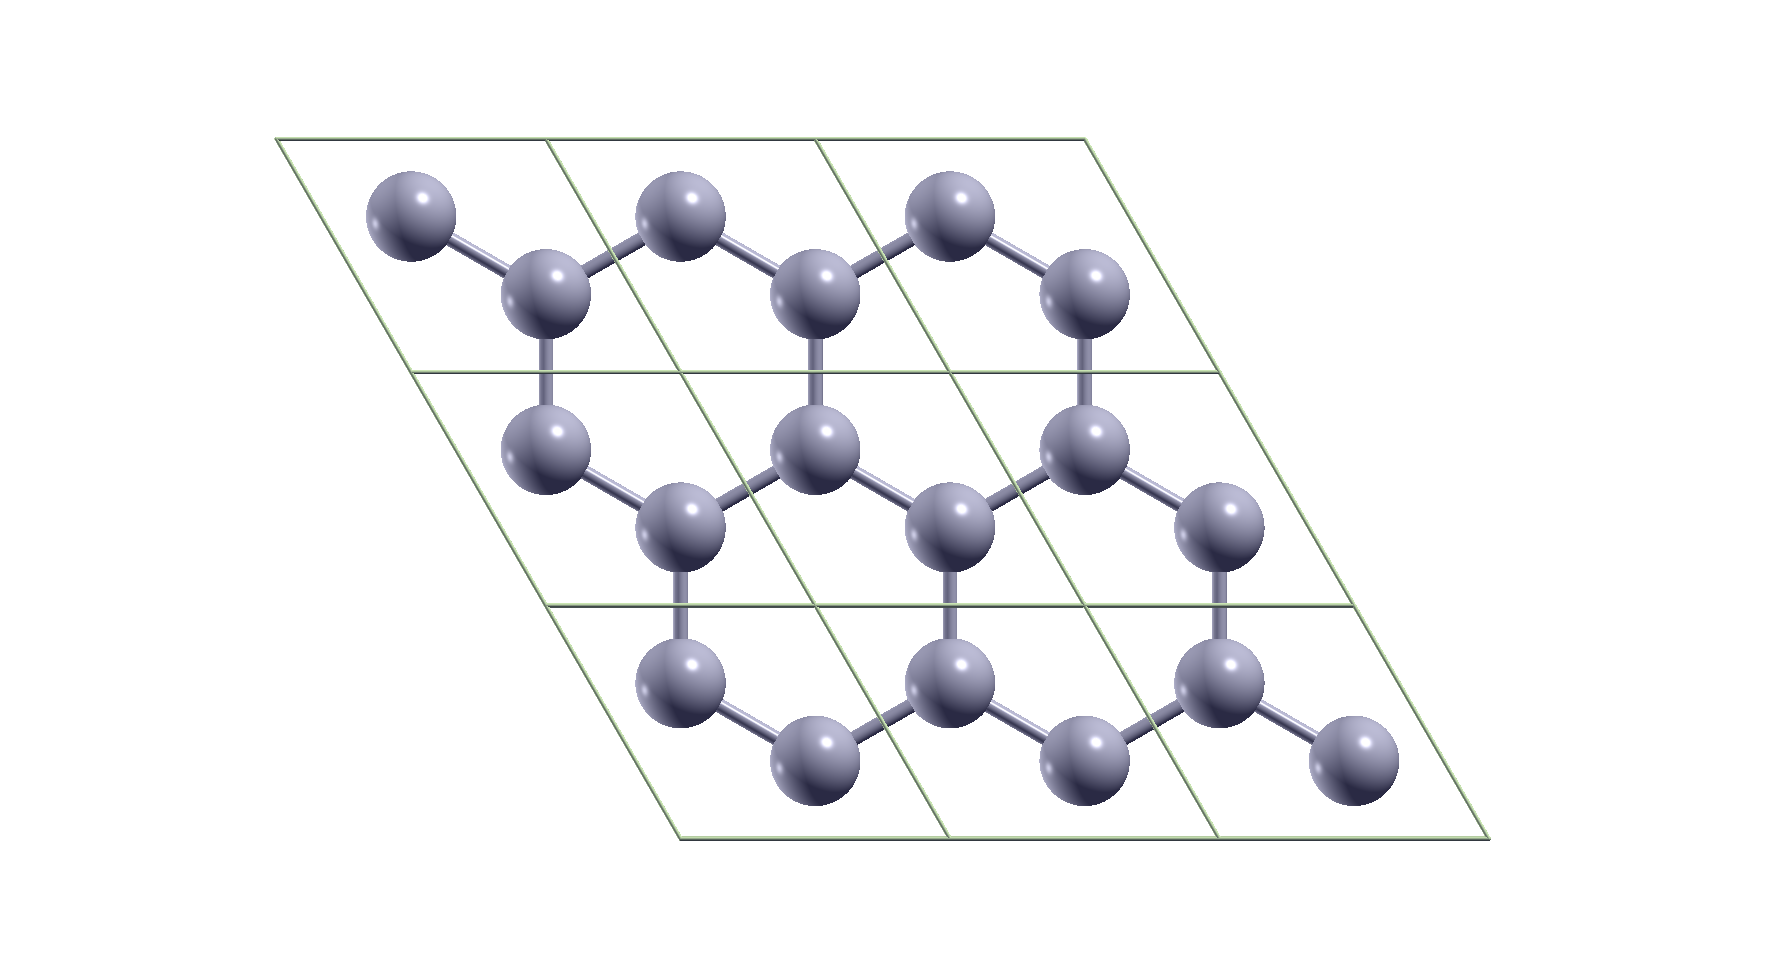
\includegraphics[width=15cm]{./gambar/pw.vc-relax.sn.png}
    \caption{Struktur optimal dari stanene}
    \label{fig:DensityofStates}
\end{figure}
Tujuan utama perhitungan \texttt{vc-relax} adalah menemukan struktur kristal yang memiliki minimum energi total dengan memvariasikan volume sel serta parameter sel seperti vektor basis. Proses optimisasi dilakukan dengan mengubah parameter-parameter ini dan menghitung ulang distribusi elektron dan energi total menggunakan metode DFT. Selama perhitungan \texttt{vc-relax}, Quantum ESPRESSO akan menyesuaikan volume sel dan parameter sel untuk mencapai keseimbangan energi minimum. Selain itu, distribusi elektron dalam struktur kristal juga akan disesuaikan untuk mencapai konvergensi yang baik. Sesuatu yang akan kita perleh dari perhtiungan ini adalah informasi penting tentang struktur kristal seperti konstanta kisi dan parameter sel optimal. Nilai optimal yang kita peroleh akan kita gunakan untuk perhitungan selanjutnya seperti mencari struktur pita maupun rapat keadaan.

Perhitungan \texttt{vc-relax} yang kami jalankan memungkinkan atom bergerak dalam arah $x$ dan $y$ saja. Perhitungan ini dapat diatur pada bagian "\texttt{cell dofree}". Setelah kalkulasi \texttt{vc-relax} dilaksanakan maka diperoleh struktur optimal untuk parameter konstanta kisi sebesar 4.68 \AA. Nilai yang kami peroleh sesuai dengan penelitian-penelitian sebelumnya. Gambar 4.3 menunjukan bentuk struktur optimal untuk Stanene


\section{Kalkulasi Sifat Elektronik}
Dalam menghitung struktur elektronik dari material stanene diperoleh struktur pita energi atau band structure dan rapat keadaan total atau density of state (rapat keadaan). Struktur pita elektronik merupakan kurva energi terhadap bilangan gelombang yang menunjukkan rentang energi yang diperbolehkan serta yang tidak diperbolehkan adanya fungsi gelombang elektron [Kittel, 2005]. Untuk mengetahui sifat material dapat diketahui dengan melihat letak potensial kimia berada dan seberapa besar \textit{band gap} yang dimiliki material. Setelah struktur optimal diperoleh maka dapat diperoleh struktur pita dan
rapat keadaan dari stanene. K-path pada zona brilloin yang digunakan adalah
Γ – K – M - Γ.

\subsection{Struktur Elektronik Stanene}
Dalam studi ini dibentuk kembali struktur pita energi dan rapat keadaan dari stanene . Hasil dari simulasi kami menunjukkan struktur pita energi stanene yang konsisten dengan penelitian sebelumnya. 

\begin{figure}[h]

\begin{subfigure}{0.5\textwidth}
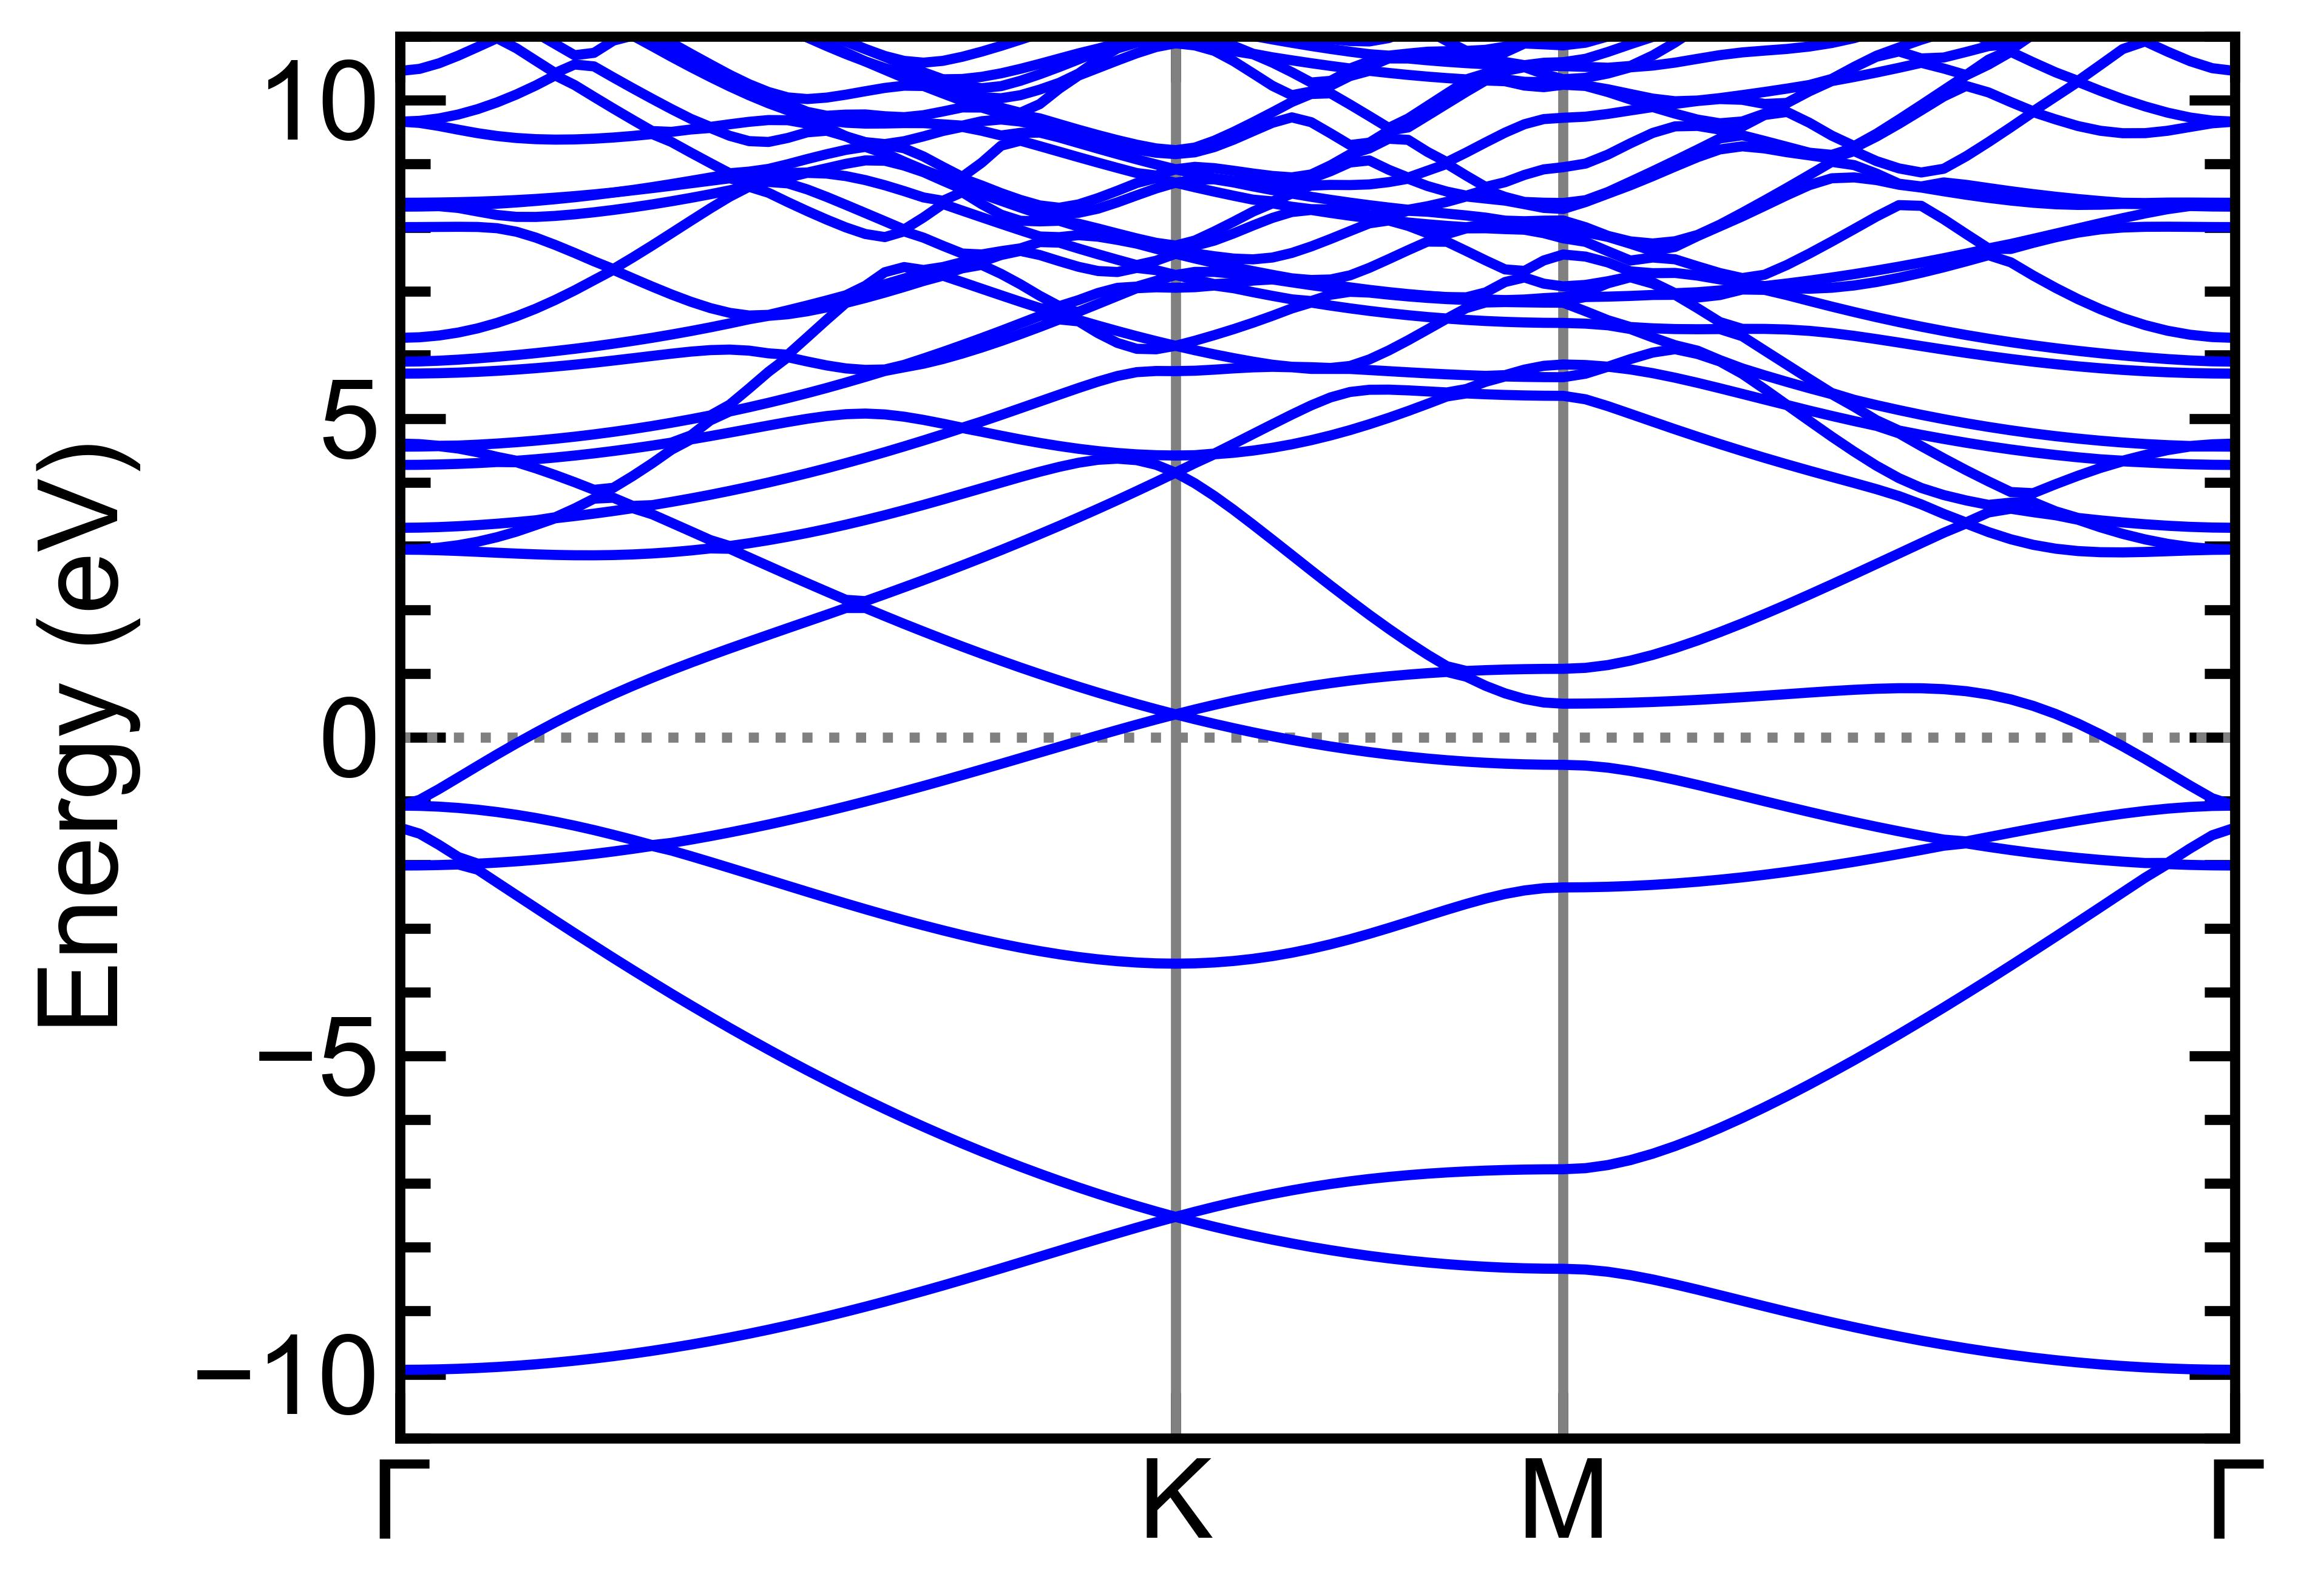
\includegraphics[width=0.9\linewidth, height=6cm]{gambar/plot_sn_bands.jpg} 
\caption{bands structure}
\label{fig:subim1}
\end{subfigure}
\begin{subfigure}{0.5\textwidth}
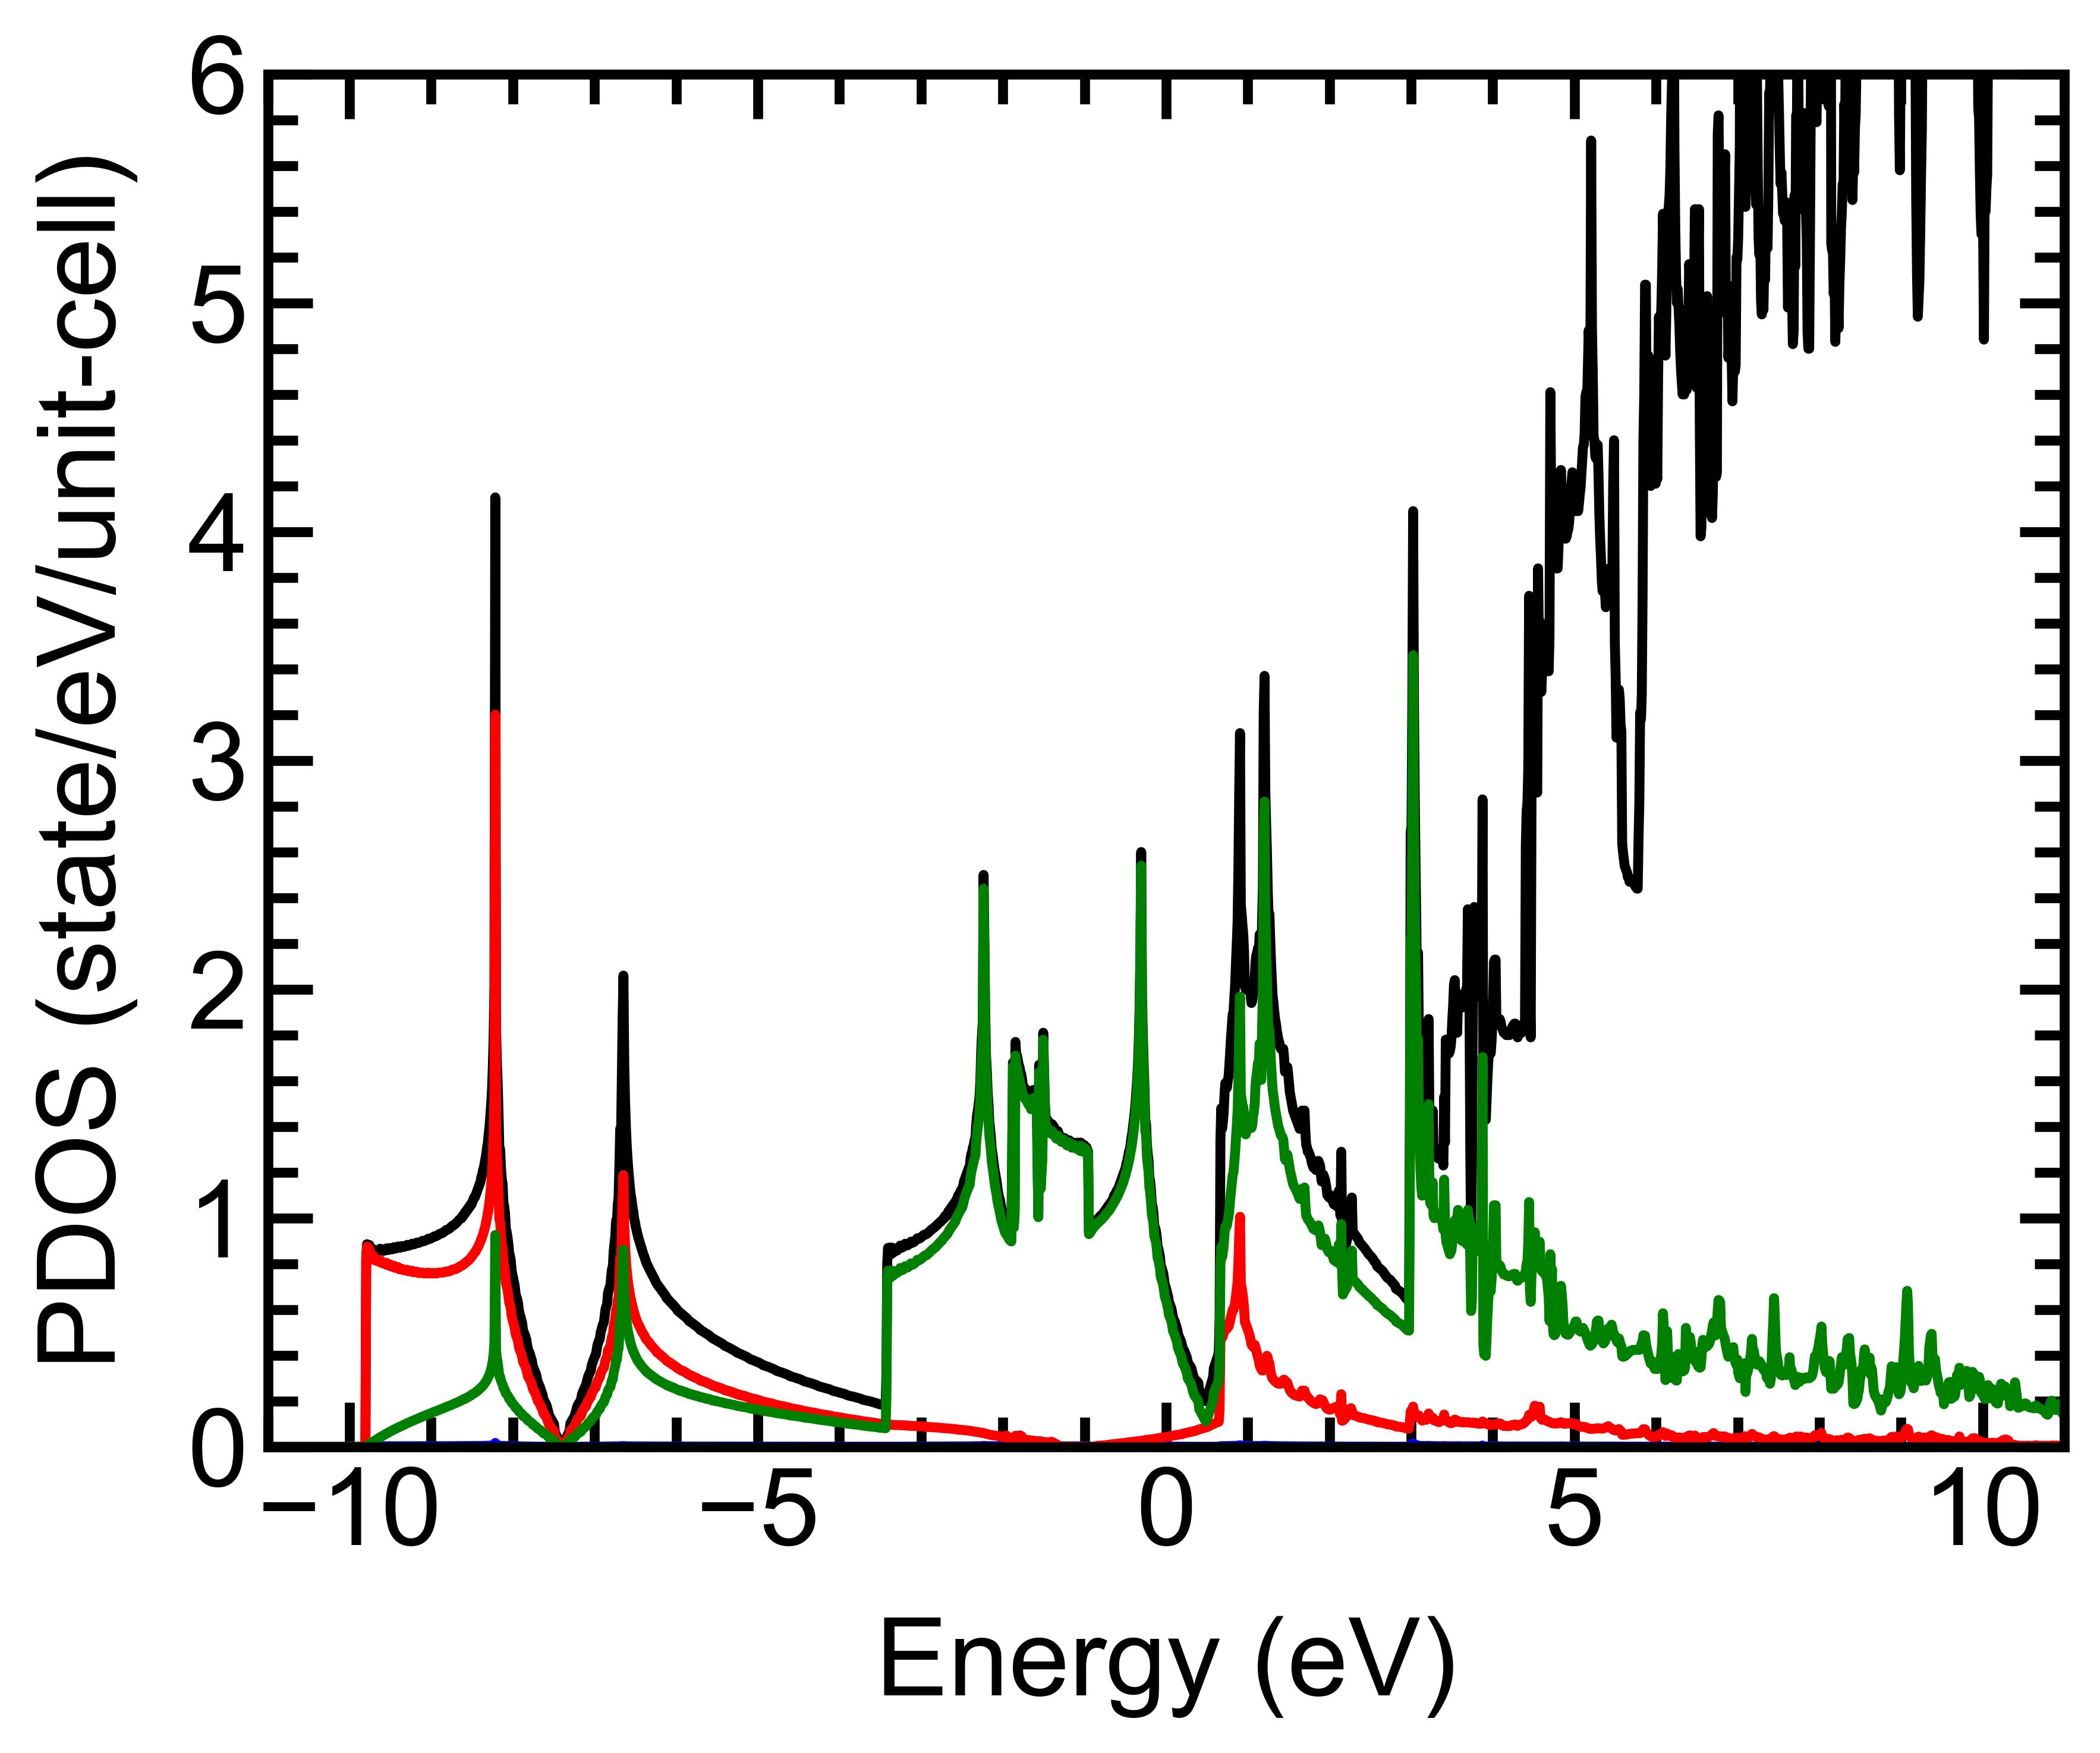
\includegraphics[width=0.9\linewidth, height=6cm]{gambar/graph_sn_pdos.jpg}
\caption{DOS dengan garis hijau adalah orbital s dan garis merah adalah orbital p}
\label{fig:subim2}
\end{subfigure}

\caption{sifat elektronik dasar dari stanene}
\label{fig:dos dan bands sn}
\end{figure}

\begin{figure}[h]
\centering
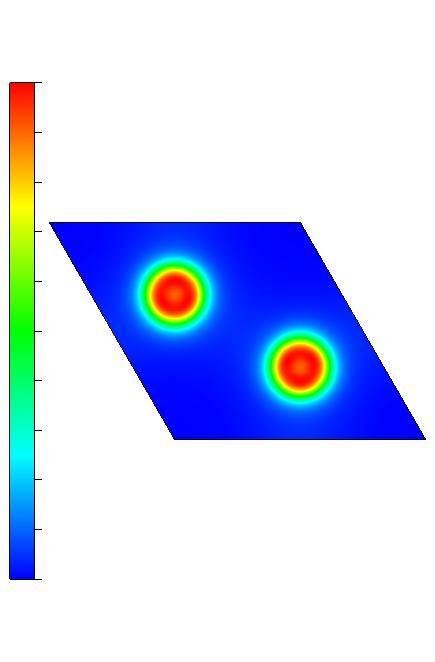
\includegraphics[width=0.5\linewidth]{gambar/sn_rho.jpg}
\caption{Rapat muatan dari stanene}
\label{fig:charge density}
\end{figure}

Seperti yang terlihat pada Gambar \ref{fig:dos dan bands sn} pita energi stanene menunjukkan dua dispersi pita, yaitu pita valensi dan pita konduksi. Pita valensi berada di bawah energi Fermi, sementara pita konduksi berada di atasnya. Selain itu, pita valensi dan konduksi saling berdekatan di titik K menunjukkan adanya tumpang tindih antara pita-pita ini yang membuat titik K memiliki Dirac cone. Fenomena Dirac cone pada titik K di stanene menurut \citep{C6RA26169H} terdiri dari orbital $5P_z$ yang menjamin stabilitas stanene dalam membentuk ikatan-$\pi$

Sementara itu rapat keadaan yang disajikan dalam grafik mengacu pada jumlah keadaan energi yang tersedia untuk elektron dalam bahan atau zat padat pada setiap tingkat energi. Ini memberikan gambaran tentang distribusi energi elektron dalam bahan dan berguna untuk memahami sifat elektronik bahan seperti konduktivitas listrik dan sifat-sifat elektronik lainnya. Rapat keadaan sering diukur dalam satuan keadaan per energi (per unit energi atau per unit massa) dan digunakan untuk menggambarkan perilaku sistem zat padat secara keseluruhan atau pada tingkat lokal.

Jenis occupation dalam file input DOS yang digunakan pada penelitian ini adalah “\texttt{tetrahedra}”. Selain \texttt{tetrahedra}, jenis occupation lain yang umum digunakan adalah \texttt{smearing} yang dibagi lagi menjadi \texttt{gaussian}, \texttt{marzari-vanderbilt}, dan \texttt{fermi-dirac}. Alasan penggunaan “tetrahedra” dalam kalkulasi DOS pada penelitian ini karena \texttt{tetrahedra} menjamin keakuratan yang lebih baik dibandingkan “smearing”. Metode tetrahedra membagi zona Brillouin menjadi tetrahedra, menghitung energi eigen di sudut-sudut setiap tetrahedron, dan secara linear menginterpolasi nilai energi eigen di dalam setiap tetrahedron untuk melakukan integrasi \citep{toriyama2021comparison}.

Pada penelitian ini juga mendapatkan distribusi kerapatan muatan dapat memberikan informasi tentang sifat ikatan antara berbagai atom. Sebagai contoh, jika muatan valensi terlokalisasi di lokasi atom, dan tidak ada muatan di antara atom, atau di ruang antar atom, maka bahan tersebut memiliki ikatan ionik. Di sisi lain, jika ada tumpukan muatan valensi di antara garis yang menghubungkan pasangan atom, maka mereka terikat secara kovalen. Sejumlah besar muatan valensi yang terdelokalisasi merupakan indikasi ikatan logam. Muatan kepadatan sistem dapat dihitung secara efisien dan divisualisasikan menggunakan alat pasca-pemrosesan yang tersedia di QE.
Pada \ref{fig:charge density} kerapatan muatan stanene diplot. Kerapatan menunjukkan hal yang signifikan yaitu berupa delokalisasi elektron yang menggambarkan kemampuan transportasi muatan terbatas.



